\section{Estimating Branch-Specific Speciation \& Extinction Rates}

\subsection{Outline}

This tutorial describes how to specify a branch-specific branching-process models in \RevBayes;
a birth-death process where diversification rates vary among branches, similar to \citep{Rabosky2014a}.
The probabilistic graphical model is given for each component of this tutorial.
The goal is to obtain estimate of branch-specific diversification rates using Markov chain Monte Carlo (MCMC).


\subsection{Requirements}
We assume that you have read and hopefully completed the following tutorials:
\begin{itemize}
\item RB\_Getting\_Started
\item RB\_Basics\_Tutorial
\item RB\_BayesFactor\_Tutorial
\item RB\_BasicDiversificationRate\_Tutorial
\end{itemize}
Note that the RB\_Basics\_Tutorial introduces the basic syntax of \Rev but does not cover any phylogenetic models.
You may skip the RB\_Basics\_Tutorial if you have some familiarity with \R.
The RB\_BayesFactor\_Tutorial introduced Bayesian model selection by means of Bayes factors, which can be skipped by readers familiar with Bayesian model selection.
We tried to keep this tutorial very basic and introduce all the language concepts and theory on the way.
You may only need the RB\_Basics\_Tutorial for a more in-depth discussion of concepts in \Rev.


%%%%%%%%
%%   Data   %%
%%%%%%%%
\section{Data and files}

We provide the data file(s) which we will use in this tutorial.
You may want to use your own data instead.
In the \cl{data} folder, you will find the following files
\begin{itemize}
\item \cl{primates\_springer.tre}: Dated primates phylogeny including 369 out of 450 species from \cite{Springer2012}.
\end{itemize}


\impmark{Open the tree \cl{data/primates\_springer.tre} in FigTree.}


\bigskip
\section{Branch-Specific Birth-Death Model}

\begin{figure}[htbp!]
\centering
\fbox{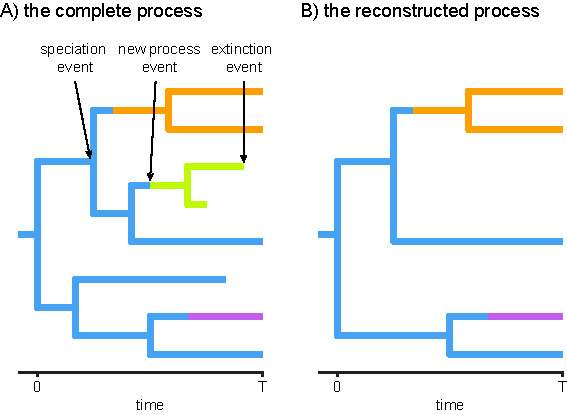
\includegraphics[width=0.7\textwidth]{\ResourcePath figures/stochastic_process_figure.pdf}}
\caption{\small Cartoon of a branch-specific birth-death process. On the left we see the full process. On the right we only see the branches of the reconstructred tree, thus missing one rate-shift event.}
\label{fig:BSBD}
\end{figure}
The basic idea behind the model is that speciation and extinction rates are allowed to vary across branches of the tree (see Figure \ref{fig:BSBD}).
Unfortunately, it is not possible to model rates drawn from a continuous distribution directly, as done for example in \BAMM, because in that case one needs to integrate over any number of possible rate shifts, any time of these shifts and most importantly over all possible new rates.
This is unfeasible to do and failure to do so has been shown to make parameter estimates unreliable.

\begin{figure}[htbp!]
\centering
\fbox{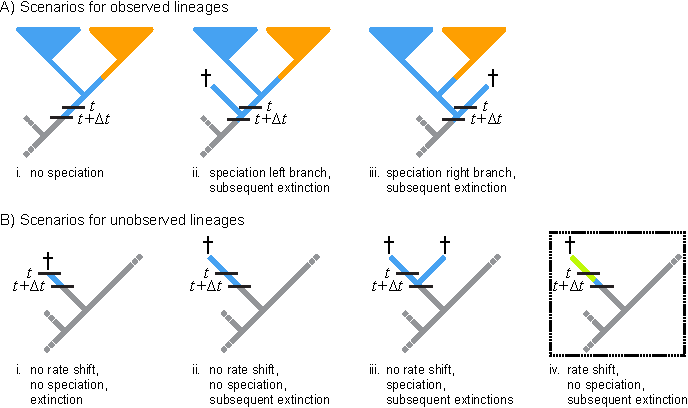
\includegraphics[width=\textwidth]{\ResourcePath figures/likelihood_figure.pdf}}
\caption{\small Cartoon of the likelihood computation using numerical integration.}
\label{fig:BSBD_likelihood}
\end{figure}
Here we adopt an approach using few discrete rate categories instead.
This allows us to numerically integrate over all possible rate categories using a system of differential equation originally described by \cite{Maddison2007} (see also \cite{FitzJohn2009} and \cite{FitzJohn2010}).
The numerical procedure beaks time into very small time interval and sums over all possible events occurring in that interval (see Figure \ref{fig:BSBD_likelihood}).

You don't need to worry about any of the technical details.
\impmark{It is important for you to realize that this model assumes that new rates at a rate-shift event are drawn from a given set (discrete) of rates.}

In \RevBayes we have two implementations (\IE distributions) for modeling a branch-specific birth-death process.
The first distribution is the \cl{dnBirthDeathMultiRate} (or its alias \cl{dnMRBDP}) and the second is the \cl{dnHeterogeneousBirthDeath} (or its alias \cl{dnHBDP}).
We have designed this tutorial so that each section can be read independently although we recommend that you work through both of them.
You will find that some parts are redundant, which is intentional to emphasize the similarities between the analysis but also to make the sections independent.


\bigskip
\section{Testing for Branch-Specific-Diversification Rates}

In this first exercise we are interested if there is diversification-rate variation among branch for our study tree.
That is, we want to see if we can reject a constant rate birth-death process.
Therefore, we don't focus on parameter estimates but instead on the marginal likelihood estimation for model testing.

\impmark{We assume that you have completed the RB\_BasicDiversificationRate\_Tutorial to estimate the marginal likelihood under a constant-rate birth-death process. If you haven't done so, then you should go back and do this now!}


\subsection{Read the tree}

Begin by reading in the observed tree. 

{\tt \begin{snugshade*}
\begin{lstlisting}
T <- readTrees("data/primates_springer.tre")[1]
\end{lstlisting}
\end{snugshade*}}

From this tree, we can get some helpful variables:
{\tt \begin{snugshade*}
\begin{lstlisting}
taxa <- T.taxa()
\end{lstlisting}
\end{snugshade*}}

Additionally, we can initialize an iterator variable for our vector of moves:
{\tt \begin{snugshade*}
\begin{lstlisting}
mi = 0
\end{lstlisting}
\end{snugshade*}}

Finally, we create a helper variable that specifies the number of discrete rate categories.
{\tt \begin{snugshade*}
\begin{lstlisting}
NUM_RATE_CATEGORIES = 4
\end{lstlisting}
\end{snugshade*}}
Using this variable we can easily change our script to use more or fewer categories and test the impact.



\subsection{Specifying the model}

\subsubsection{Priors on rates}
\begin{figure}[htbp!]
\centering
\fbox{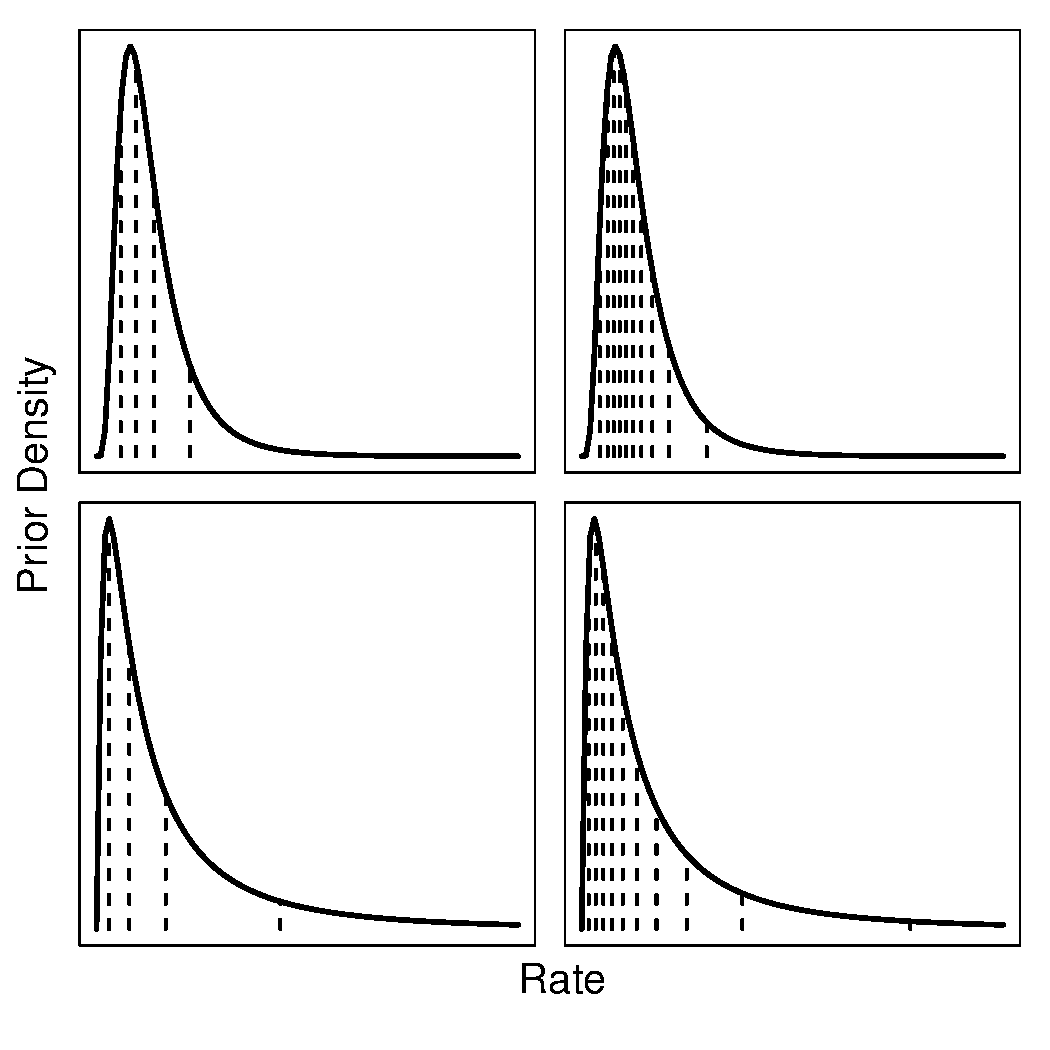
\includegraphics[width=\textwidth]{\ResourcePath figures/discretized_lognormal.pdf}}
\caption{\small Discretization of a lognormal distribution. The two left figures have 4 rate categories and the two right plots have 10 rate categories. The top plots have the 95\% probability interval spanning one order of magnitude (\cl{sd} $=0.587405$) and the bottom plots have the 95\% probability interval spanning two orders of magnitude (\cl{sd} $=2*0.587405$)}
\label{fig:BSBD_likelihood}
\end{figure}
Instead of using a continuous probability distribution we will use a discrete approximation of the distribution, as done for modeling rate variation across sites \citep{Yang1994a} and for modeling relaxed molecular clocks \citep{Drummond2006}.
That means, we assume that the speciation rates are drawn from one of the $N$ quantiles of the lognormal distribution.
For this we will use the function \cl{fnDiscretizeDistribution} which takes in a distribution as its first argument and the number of quantile as the second argument.
The return value is a vector of quantiles.
We use it as a deterministic variable and every time the parameters of the base distribution (\IE the lognormal distribution in our case) change the quantiles will update automatically as well.
Thus we only need to specify parameters for our base distribution, the lognormal distribution.
We choose a stochastic variable for the mean parameter of the lognormal distribution drawn from another lognormal prior distribution.
We fix the prior mean on this mean diversification rate on our expected diversification rate, which is $\ln( \ln(\frac{\#Taxa}{2})/age )$.
Remember that the median of a lognormal distribution is equal to the exponential of the mean parameter.
This is why we used a log-transform of the actual mean.
This prior density is analogous to the prior on the diversification rate in the constant-rate birth-death process.
{\tt \begin{snugshade*}
\begin{lstlisting}
diversification_prior_mean <- ln( ln(450.0/2.0) / T.rootAge() )
diversification_mean ~ dnLognormal(mean=diversification_prior_mean, sd=0.587405)
moves[++mi] = mvScale(diversification_mean,lambda=1,tune=true,weight=5)
\end{lstlisting}
\end{snugshade*}}
Additionally, we choose a fixed standard deviation of $0.587405*2$ for the speciation rates because it represents two orders of magnitude variance in the rate categories.
{\tt \begin{snugshade*}
\begin{lstlisting}
diversification_sd <- 0.587405*2
diversification := fnDiscretizeDistribution( dnLognormal(ln(diversification_mean), diversification_sd), NUM_RATE_CATEGORIES )
\end{lstlisting}
\end{snugshade*}}
For each of the speciation rate categories we need a extinction rate category.
We are completely free to choose how we construct these rate categories.
For example, we could chose a similar discretization of a lognormal distribution using its quantiles to provide different extinction rate categories.
The only drawback of this approach is that low speciation rates are paired by definition with low extinction rates and high extinction rates are paired with high extinction rates.
This is because rates are pared by their index, thus the speciation rate with index $j$ is paired with the extinction rate with index $j$.
We could avoid this by estimating $N$ independent rate categories instead of assuming that the rate categories are computed by the quantile function.

Another option is to simply assume that the relative extinction rate is equal for all rate category.
We use this model choice in this exercise.
Hence, we only need to create one random variable for the relative extinction rate.
{\tt \begin{snugshade*}
\begin{lstlisting}
turnover_prior_mean <- ln( ln(450.0/2.0) / T.rootAge() )
turnover_mean ~ dnLognormal(mean=turnover_prior_mean,sd=0.587405*2) 
moves[++mi] = mvScale(turnover_mean,lambda=1.0,tune=true,weight=3.0)
\end{lstlisting}
\end{snugshade*}}
Then we multiply each speciation rate category by the relative extinction rate to obtain the extinction rates per rate category.
{\tt \begin{snugshade*}
\begin{lstlisting}
turnover := fnDiscretizeDistribution( dnLognormal(ln(turnover_mean), 0.587405), NUM_RATE_CATEGORIES )
\end{lstlisting}
\end{snugshade*}}
Finally, we transform the diversification and turnover rate into the speciation and extinction rate parameters, as required by the birth-death process.
{\tt \begin{snugshade*}
\begin{lstlisting}
speciation := diversification + turnover
extinction := turnover 
\end{lstlisting}
\end{snugshade*}}

Next, we need a rate parameter for the rate-shifts events.
Again, there we do not have much prior information about this rate and choose an exponential distribution with rate 1.0.
As usual for rate parameter, we apply a scaling move to the \cl{event\_rate} variable.
{\tt \begin{snugshade*}
\begin{lstlisting}
event_rate ~ dnExponential(1.0)
moves[++mi] = mvScale(event_rate,lambda=1,tune=true,weight=5)
\end{lstlisting}
\end{snugshade*}}

Additionally, we need a rate-matrix parameter providing the relative rates between rate categories.
In this case we simply use equal rates between each rate category; and thus use the Jukes-Cantor rate matrix.
You could, for example, also use an ordered rate matrix where the process needs to go through rate 2 before going to rate 3 when starting in rate 1.
{\tt \begin{snugshade*}
\begin{lstlisting}
rate_matrix <- fnJC( NUM_RATE_CATEGORIES )
\end{lstlisting}
\end{snugshade*}}
Furthermore, we need prior probabilities for the process being in either rate category at the root.
Given our lack of prior knowledge we create a flat prior distribution giving each rate category equal weight.
We do this by create a constant variable using the simplex function.
{\tt \begin{snugshade*}
\begin{lstlisting}
rate_category_prior <- simplex( rep(1,NUM_RATE_CATEGORIES) )
\end{lstlisting}
\end{snugshade*}}



\subsubsection{Incomplete Taxon Sampling}

We know that we have sampled 367 out of 450 living primate species. 
To account for this we can set the sampling parameter as a constant node with a value of 369/450
{\tt \begin{snugshade*}
\begin{lstlisting}
rho <- T.ntips()/450
\end{lstlisting}
\end{snugshade*}}


\subsubsection{Root age}

The birth-death process requires a parameter for the root age.
In this exercise we use a fix tree and thus we know the age of the tree.
Hence, we can get the value for the root from the \citet{Springer2012} tree.
{\tt \begin{snugshade*}
\begin{lstlisting}
root_time <- T.rootAge()
\end{lstlisting}
\end{snugshade*}}

\subsubsection{The time tree}

Now we have all of the parameters we need to specify the full episodic birth-death model. 
We initialize the stochastic node representing the time tree.
{\tt \begin{snugshade*}
\begin{lstlisting}
timetree ~ dnMRBDP(lambda=speciation, mu=extinction, rootAge=root, rho=rho, Q=rate_matrix, pi=rate_category_prior, delta=event_rate, taxa=taxa )
\end{lstlisting}
\end{snugshade*}}
And then we attach data to it.
{\tt \begin{snugshade*}
\begin{lstlisting}
timetree.clamp(T)
\end{lstlisting}
\end{snugshade*}}



Finally, we create a workspace object of our whole model using the \cl{model()} function. 
{\tt \begin{snugshade*}
\begin{lstlisting}
mymodel = model(speciation)
\end{lstlisting}
\end{snugshade*}}

The \cl{model()} function traversed all of the connections and found all of the nodes we specified. 


\subsection{Running a marginal likelihood estimation}

\subsubsection{Specifying Monitors}

For the marginal likelihood analysis we don't necessarily need monitors because we are not going to look into the samples.
However, as good practice we still define our two standard monitors: the model monitor and a screen monitor
{\tt \begin{snugshade*}
\begin{lstlisting}
monitors[1] = mnModel(filename="output/primates_MRBD.log",printgen=10, separator = TAB)
monitors[2] = mnScreen(printgen=10, diversification_mean, turnover)
\end{lstlisting}
\end{snugshade*}}

\subsubsection{Initializing and Running the MCMC Simulation}

\impmark{If you don't feel comfortable with Bayesian model selection anymore, then have a look at the \href{https://github.com/revbayes/revbayes_tutorial/raw/master/tutorial_TeX/RB_BayesFactor_Tutorial/RB_BayesFactor_Tutorial.pdf}{RB\_BayesFactor\_Tutorial} again.}


First, we create the variable containing the power posterior. 
This requires us to provide a model and vector of moves, as well as an output file name. 
The \cl{cats} argument sets the number of power steps.
{\tt \begin{snugshade*}
\begin{lstlisting}
pow_p = powerPosterior(mymodel, moves, "output/MRBD_powp.out", cats=100) 
\end{lstlisting}
\end{snugshade*}}

We can start the power posterior by first burning in the chain and and discarding the first 5000 states.  
{\tt \begin{snugshade*}
\begin{lstlisting}
pow_p.burnin(generations=5000,tuningInterval=200)
\end{lstlisting}
\end{snugshade*}}

Now execute the run with the \cl{.run()} function:
{\tt \begin{snugshade*}
\begin{lstlisting}
pow_p.run(generations=2000)  
\end{lstlisting}
\end{snugshade*}}

Once the power posteriors have been saved to file, create a stepping stone sampler. 
This function can read any file of power posteriors and compute the marginal likelihood using stepping-stone sampling. 
{\tt \small \begin{snugshade*}
\begin{lstlisting}
ss = steppingStoneSampler(file="output/MRBD_powp.out", powerColumnName="power", likelihoodColumnName="likelihood")
\end{lstlisting}
\end{snugshade*}}

Compute the marginal likelihood under stepping-stone sampling using the member function \cl{marginal()} of the \cl{ss} variable and record the value in Table \ref{tab:ss}.
{\tt \begin{snugshade*}
\begin{lstlisting}
ss.marginal() 
\end{lstlisting}
\end{snugshade*}}

Path sampling is an alternative to stepping-stone sampling and also takes the same power posteriors as input. 
{\tt \small \begin{snugshade*}
\begin{lstlisting}
ps = pathSampler(file="output/MRBD_powp.out", powerColumnName="power", likelihoodColumnName="likelihood")
\end{lstlisting}
\end{snugshade*}}

Compute the marginal likelihood under stepping-stone sampling using the member function \cl{marginal()} of the \cl{ps} variable and record the value in Table \ref{tab:ss}.
{\tt \begin{snugshade*}
\begin{lstlisting}
ps.marginal() 
\end{lstlisting}
\end{snugshade*}}


\impmark{The \Rev file for performing this analysis: \href{https://github.com/revbayes/revbayes_tutorial/raw/master/RB_DiversificationRateBranchSpecific_Tutorial/RevBayes_scripts/ml_MRBD.Rev}{\cl{ml\_MRBD.Rev}}.}


\subsection{Exercise 1}

\begin{itemize}
\item Enter the marginal likelihood estimate from the previous exercise on the constant-rate birth-death process in the table below.
\item Compute the marginal likelihood under the 2-rate model, \IE set the NUM\_Rate\_CATEGORIES variable to 2.
\item Repeat the estimation of the marginal likelihoods with other number of rate categories to fill out the table.
\item What is the most supported model? Can we reject the constant-rate birth-death process?
\end{itemize}

\begin{Form}
\begin{table}[h!]
\centering
\caption{\small Marginal likelihoods and Bayes factors$^*$.}
\begin{tabular}{l c c c c}
\hline
\multicolumn{1}{l}{\textbf{Estimate}} & \multicolumn{1}{r}{\hspace{3mm}} & \multicolumn{1}{c}{\textit{Stepping-stone}} & \multicolumn{1}{r}{\hspace{3mm}} & \multicolumn{1}{c}{\textit{Path sampling}} \\ 
\hline
Marginal likelihood constant-rate ($N=0$) & \hspace{15mm} & \TextField[name=ml7,backgroundcolor={.85 .85 .85},color={1 0 0},height=4ex]{}  & \hspace{15mm} & \TextField[name=ml8,backgroundcolor={.85 .85 .85},color={0 0 1},height=4ex]{} \\
\hline
Marginal likelihood two rate ($N=2$) & \hspace{3mm} & \TextField[name=ml9,backgroundcolor={.85 .85 .85},color={1 0 0},height=4ex]{} & \hspace{3mm} & \TextField[name=ml10,backgroundcolor={.85 .85 .85},color={0 0 1},height=4ex]{} \\
\hline
Marginal likelihood four rate ($N=4$) & \hspace{3mm} & \TextField[name=ml9,backgroundcolor={.85 .85 .85},color={1 0 0},height=4ex]{} & \hspace{3mm} & \TextField[name=ml10,backgroundcolor={.85 .85 .85},color={0 0 1},height=4ex]{} \\
\hline
Marginal likelihood six rate ($N=6$) & \hspace{3mm} & \TextField[name=ml9,backgroundcolor={.85 .85 .85},color={1 0 0},height=4ex]{} & \hspace{3mm} & \TextField[name=ml10,backgroundcolor={.85 .85 .85},color={0 0 1},height=4ex]{} \\
\hline
Marginal likelihood eight rate ($N=8$) & \hspace{3mm} & \TextField[name=ml9,backgroundcolor={.85 .85 .85},color={1 0 0},height=4ex]{} & \hspace{3mm} & \TextField[name=ml10,backgroundcolor={.85 .85 .85},color={0 0 1},height=4ex]{} \\
\hline
Marginal likelihood ten rate ($N=10$) & \hspace{3mm} & \TextField[name=ml9,backgroundcolor={.85 .85 .85},color={1 0 0},height=4ex]{} & \hspace{3mm} & \TextField[name=ml10,backgroundcolor={.85 .85 .85},color={0 0 1},height=4ex]{} \\
\hline
Supported model? & \hspace{3mm} &  \TextField[name=ml13,backgroundcolor={1 .85 .85},color={1 0 0},height=4ex]{} & \hspace{3mm} & \TextField[name=ml14,backgroundcolor={.85 .85 1},color={0 0 1},height=4ex]{} \\
\hline
{\footnotesize{$^*$you can edit this table}}\\
\end{tabular}
\label{tab:ss}
\end{table}
\end{Form}








\bigskip
\section{Estimating Branch-Specific Diversification Rates}

In this second analysis we are interested in estimating the branch-specific diversification rates.
We are going to use a very similar model to the model described in the previous section.
However, now we are going to use the \cl{dnHBDP} distribution instead which will require some slightly different parameterization and moves.
The main difference, as mentioned above, is that the \cl{dnHBDP} uses a data augementation scheme to add the rate-shift events onto the tree.

\subsection{Read the tree}

Begin by reading in the observed tree. 

{\tt \begin{snugshade*}
\begin{lstlisting}
T <- readTrees("data/primates_springer.tre")[1]
\end{lstlisting}
\end{snugshade*}}

From this tree, we can get some helpful variables:
{\tt \begin{snugshade*}
\begin{lstlisting}
taxa <- T.taxa()
\end{lstlisting}
\end{snugshade*}}

Additionally, we can initialize an iterator variable for our vector of moves:
{\tt \begin{snugshade*}
\begin{lstlisting}
mi = 0
\end{lstlisting}
\end{snugshade*}}

Finally, we create a helper variable that specifies the number of discrete rate categories.
{\tt \begin{snugshade*}
\begin{lstlisting}
NUM_RATE_CATEGORIES = 10
\end{lstlisting}
\end{snugshade*}}
Using this variable we can easily change our script to use more or fewer categories and test the impact.



\subsection{Specifying the model}

\subsubsection{Priors on rates}
Analogous to the previous section we will set up the rate categories using the exact same model and \Rev syntax.
Thus, we create first our hyper-prior on the mean diversification rate, which is drawn from a lognormal distribution.
{\tt \begin{snugshade*}
\begin{lstlisting}
diversification_prior_mean <- ln( ln(450.0/2.0) / T.rootAge() )
diversification_mean ~ dnLognormal(mean=diversification_prior_mean, sd=0.587405)
moves[++mi] = mvScale(diversification_mean,lambda=1,tune=true,weight=5)
\end{lstlisting}
\end{snugshade*}}
Additionally, we choose a fixed standard deviation of $0.587405*2$ for the speciation rates because it represents two orders of magnitude variance in the rate categories.
{\tt \begin{snugshade*}
\begin{lstlisting}
diversification_sd <- 0.587405*2
diversification := fnDiscretizeDistribution( dnLognormal(ln(diversification_mean), diversification_sd), NUM_RATE_CATEGORIES )
\end{lstlisting}
\end{snugshade*}}
We define the prior on the turnover rate in the same way as we did for the diversification rate, with the only difference that we allow for two orders of magnitude of uncertainty.
{\tt \begin{snugshade*}
\begin{lstlisting}
turnover_prior_mean <- ln( ln(450.0/2.0) / T.rootAge() )
turnover_mean ~ dnLognormal(mean=turnover_prior_mean,sd=0.587405*2) 
moves[++mi] = mvScale(turnover_mean,lambda=1.0,tune=true,weight=3.0)
\end{lstlisting}
\end{snugshade*}}
Then we multiply each speciation rate category by the relative extinction rate to obtain the extinction rates per rate category.
{\tt \begin{snugshade*}
\begin{lstlisting}
turnover := fnDiscretizeDistribution( dnLognormal(ln(turnover_mean), 0.587405), NUM_RATE_CATEGORIES )
\end{lstlisting}
\end{snugshade*}}
Finally, we transform the diversification and turnover rate into the speciation and extinction rate parameters, as required by the birth-death process.
{\tt \begin{snugshade*}
\begin{lstlisting}
speciation := diversification + turnover
extinction := turnover 
\end{lstlisting}
\end{snugshade*}}

Next, we need a rate parameter for the rate-shifts events.
Again, there we do not have much prior information about this rate and choose an exponential distribution with rate 1.0.
As usual for rate parameter, we apply a scaling move to the \cl{event\_rate} variable.
{\tt \begin{snugshade*}
\begin{lstlisting}
event_rate ~ dnExponential(1.0)
moves[++mi] = mvScale(event_rate,lambda=1,tune=true,weight=5)
\end{lstlisting}
\end{snugshade*}}

Additionally, we need a parameter for the category of the process at root.
We use a uniform prior distribution on the indices 1 to $N$ since we do not have any prior information in which rate category the process is at the root.
The move for this random variable is a random integer walk because the random variable is defined only on the indices (\CF with real number).
{\tt \begin{snugshade*}
\begin{lstlisting}
root_category ~ dnUniformNatural(1,NUM_RATE_CATEGORIES)
moves[++mi] = mvRandomIntegerWalk(root_category,weight=1)
\end{lstlisting}
\end{snugshade*}}



\subsubsection{Incomplete Taxon Sampling}

We know that we have sampled 367 out of 450 living primate species. 
To account for this we can set the sampling parameter as a constant node with a value of 369/450
{\tt \begin{snugshade*}
\begin{lstlisting}
rho <- T.ntips()/450
\end{lstlisting}
\end{snugshade*}}


\subsubsection{Root age}

The birth-death process requires a parameter for the root age.
In this exercise we use a fix tree and thus we know the age of the tree.
Hence, we can get the value for the root from the \citet{Springer2012} tree.
{\tt \begin{snugshade*}
\begin{lstlisting}
root_time <- T.rootAge()
\end{lstlisting}
\end{snugshade*}}

\subsubsection{The time tree}

Now we have all of the parameters we need to specify the full episodic birth-death model. 
We initialize the stochastic node representing the time tree.
{\tt \begin{snugshade*}
\begin{lstlisting}
timetree ~ dnHBDP(lambda=speciation, mu=extinction, rootAge=root_time, rho=rho, rootState=root_category, delta=event_rate, taxa=taxa )
\end{lstlisting}
\end{snugshade*}}
And then we attach data to it.
{\tt \begin{snugshade*}
\begin{lstlisting}
timetree.clamp(T)
\end{lstlisting}
\end{snugshade*}}

This specific implementation of the branch-specific birth-death process augments the tree with rate-shift events.
In order to sample the number, the location, and the types of the rate-shift events, we have to apply special moves to the tree.
These moves will not change the tree but only the augmented rate-shift events.
We use a \cl{mvBirthDeathEvent} to add and remove events, a \cl{mvEventTimeSlide} and \cl{mvEventTimeBeta} move to change the time and location of the events, 
and a \cl{mvDiscreteEventCategoryRandomWalk} to change the new rate categories after an event occured.
{\tt \begin{snugshade*}
\begin{lstlisting}
moves[++mi] = mvBirthDeathEvent(timetree,weight=2)
moves[++mi] = mvEventTimeSlide(timetree,weight=2)
moves[++mi] = mvEventTimeBeta(timetree,weight=2)
moves[++mi] = mvDiscreteEventCategoryRandomWalk(timetree,weight=2)
\end{lstlisting}
\end{snugshade*}}

In the first place we are interested in the branch-specific rates.
So far we do not have any variables that directly give us the number of rate-shift events per branch or the rates per branch.
Fortunately, we can construct deterministic variables and query these properties from the tree.
These function are made available by the branch-specific birth-death process distribution.
{\tt \begin{snugshade*}
\begin{lstlisting}
num_events := timetree.numberEvents()
avg_lambda := timetree.averageSpeciationRate()
avg_mu     := timetree.averageExtinctionRate()

total_num_events := sum( num_events )
\end{lstlisting}
\end{snugshade*}}


Finally, we create a workspace object of our whole model using the \cl{model()} function. 
{\tt \begin{snugshade*}
\begin{lstlisting}
mymodel = model(speciation)
\end{lstlisting}
\end{snugshade*}}

The \cl{model()} function traversed all of the connections and found all of the nodes we specified. 


\subsection{Running an MCMC analysis}

\subsubsection{Specifying Monitors}

For our MCMC analysis, we need to set up a vector of \textit{monitors} to record the states of our Markov chain. 
First, we will initialize the model monitor using the \cl{mnModel} function. This creates a new monitor variable that will output the states for all model parameters when passed into a MCMC function. 
{\tt \begin{snugshade*}
\begin{lstlisting}
monitors[1] = mnModel(filename="output/primates_BSBD.log",printgen=10, separator = TAB)
\end{lstlisting}
\end{snugshade*}}

Additionally, we create an extended-newick monitor.
The extended-newick monitor writes the tree to a file and adds parameter values to the branches and/or nodes of the tree.
We can thus print the tree with the average speciation and extinction rates at the branches into a files.
We will need this file later to estimate and visualize the posterior distribution of the rates at the branches.
{\tt \begin{snugshade*}
\begin{lstlisting}
monitors[2] = mnExtNewick(filename="output/primates_BSBD.trees", isNodeParameter=FALSE, printgen=10, separator = TAB, tree=timetree, avg_lambda, avg_mu)
\end{lstlisting}
\end{snugshade*}}

Finally, create a screen monitor that will report the states of specified variables to the screen with \cl{mnScreen}:
{\tt \begin{snugshade*}
\begin{lstlisting}
monitors[3] = mnScreen(printgen=10, event_rate, mean_speciation, root_category, total_num_events)
\end{lstlisting}
\end{snugshade*}}

\subsubsection{Initializing and Running the MCMC Simulation}

With a fully specified model, a set of monitors, and a set of moves, we can now set up the MCMC algorithm that will sample parameter values in proportion to their posterior probability. The \cl{mcmc()} function will create our MCMC object:
{\tt \begin{snugshade*}
\begin{lstlisting}
mymcmc = mcmc(mymodel, monitors, moves)
\end{lstlisting}
\end{snugshade*}}

First, we will run a pre-burnin to tune the moves and to obtain starting values from the posterior distribution.
{\tt \begin{snugshade*}
\begin{lstlisting}
mymcmc.burnin(generations=10000,tuningInterval=200)
\end{lstlisting}
\end{snugshade*}}


Now, run the MCMC:
{\tt \begin{snugshade*}
\begin{lstlisting}
mymcmc.run(generations=50000)
\end{lstlisting}
\end{snugshade*}}

When the analysis is complete, you will have the monitored files in your output directory.
You can then visualize the branch-specific rates by attaching them to the tree.
This is actually done automatically in our \cl{mapTree} function.
{\tt \begin{snugshade*}
\begin{lstlisting}
treetrace = readTreeTrace("output/primates_BSBD.trees", treetype="clock")
map_tree = mapTree(treetrace,"output/primates_BSBD_MAP.tree")
\end{lstlisting}
\end{snugshade*}}
Now you can open the tree in \FigTree.


\impmark{The \Rev file for performing this analysis: \href{https://github.com/revbayes/revbayes_tutorial/raw/master/RB_DiversificationRateBranchSpecific_Tutorial/RevBayes_scripts/mcmc_BSBD.Rev}{\cl{mcmc\_BSBD.Rev}}.}


\subsection{Exercise}

\begin{itemize}
\item Run an MCMC simulation to estimate the posterior distribution of the speciation rate and extinction rate.
\item Visualize the branch-specific rates in \FigTree.
\item Do you see evidence for rate decreases or increases? What is the general trend?
\item Run the analysis using a different number of categories, \EG 5 or 50. How do the rates change?
\item Modify the model by specifying a prior on the log-diversification and log-turnover rate and then estimate the diversification rates through time. Do you see any differences in the estimates? 
\end{itemize}




\bibliographystyle{sysbio}
\bibliography{\GlobalResourcePath refs}
